\section{Exercise 4}

To answer the question posed in the task, we used the matplotlib plotting library for the python programming language.\\\\
For this, we initialize the pseudo-random number generator with the \texttt{seed()} function and then randomly pick a 1 or -1 with the \texttt{choice()} function from the random library for the given N number of times. The chosen number is then added to a \texttt{value} variable to display the tendency toward heads or tails.\\
For the gathered data, we track the following things:
\begin{enumerate}
    \item total amount of heads \& tails
    \item maximum \& minimum \texttt{value}
    \item longest streak of heads \& tails
    \item iterations/coin throws where \texttt{value} 0 is reached
\end{enumerate}
The data is then displayed using two graphs (and the console). First, we plot the development of the \texttt{value} variable in regards to the coin throws, as can be see in \autoref{fig1}. Second, we plot the total amount of heads and tails in a bar graph, to display the ratio, as can be seen in \autoref{fig2}.\\\\
When experimenting with this setup, we found the following regarding the tracked parameters for increasingly high sample sizes N. The first and most important observation was the 'law of large numbers' (probability theory), as we noticed that the \texttt{value} variable tended more toward 0 for larger sample sizes, as can be seen in figures 1, 3 and 4. While \autoref{fig1} has a final value of 27, \autoref{3} and \autoref{4} have final values of -19 and 179 respectively, which is a much smaller deviation from 0, when taking sample size into account. This can be seen especially well when comparing \autoref{2}, \autoref{5} and \autoref{6}, which show the ratio being closer to 1:1 for higher sample sizes. However, it is important to mention that the deviation is only reduced when taking the sample size into account. In absolute values, the devation actually increases (179 for N = 1,000,000 and 27 for N = 1,000). This can also be observed when comparing the amount of times the \texttt{value} 0 is reached (and when) for higher sample sizes. For \autoref{fig1} the \texttt{value} 0 is reached 48 times within the 1,000 iterations. However, in \autoref{fig4} in the last 1,000 iterations, the \texttt{value} 0 is only reached 7 times.\\\\
The last two observations were that for higher sample sizes, higher and lower maximum and minimum values respectively and longer streaks are reached. In \autoref{fig1} the maximum \texttt{value} is 28 and the minimum \texttt{value} is -7, while in \autoref{fig3} they are 182 and -86 and in \autoref{fig4}, they are 576 and -732 respectively. Similarly, the longest streak for heads is 10 in \autoref{fig1} and 21 in \autoref{fig3}.\\
While both of these parameters become more extreme, they are not proportional to the higher sample sizes as higher deviations become exponentially more unlikely (as a random walk this coin throwing simulation follows a normal distribution).\\\\
Moreover, to display the observed tendency towards the \texttt{value} 0, we can also plot multiple simulations in one graph, as can be seen in \autoref{fig7}. This figure shows three simulations close to 0 and two others with a slight tendency towards heads and tails, respectively.
\\\\
Lastly, until now, we have simulated the coin throwing with an unweighted coin. However, if we were to change the probabilities even slightly in favor of heads, the tendency toward 0 is replaced with a tendency toward heads, as can be seen in \autoref{8}, \autoref{9}, \autoref{fig10} and \autoref{fig11}.

\begin{figure}
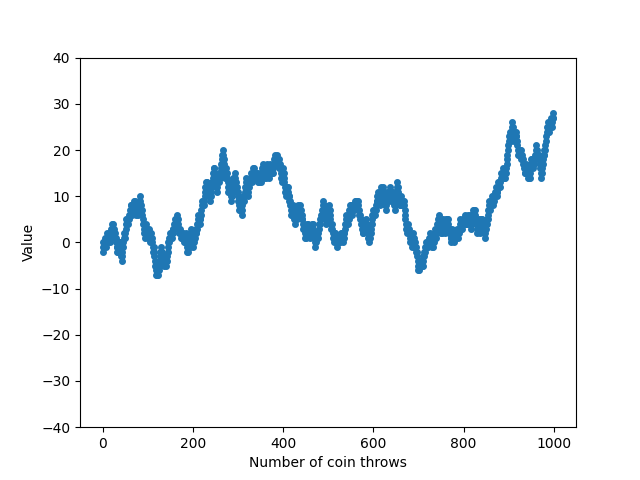
\includegraphics[scale=0.7]{./matplotlib_graphs/Figure_1.png}
\centering
\caption{Plot shows development of \texttt{value} for sample size of N = 1,000} \label{fig1}
\end{figure}

\begin{figure}
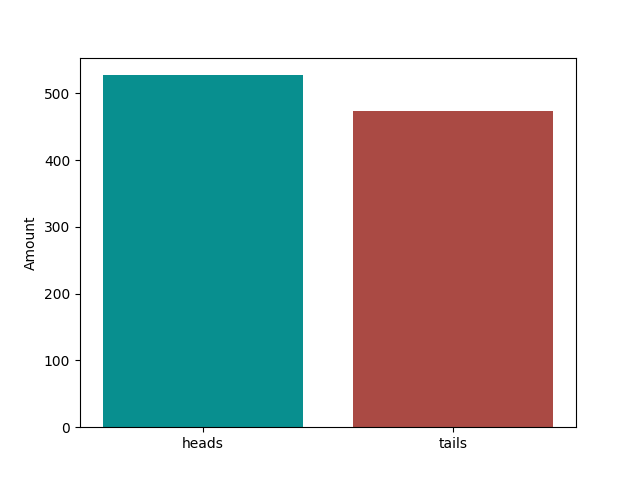
\includegraphics[scale=0.7]{./matplotlib_graphs/Figure_1_bar.png}
\centering
\caption{Bar graph shows ration of heads and tails for sample size of N = 1,000} \label{fig2}
\end{figure}

\begin{figure}
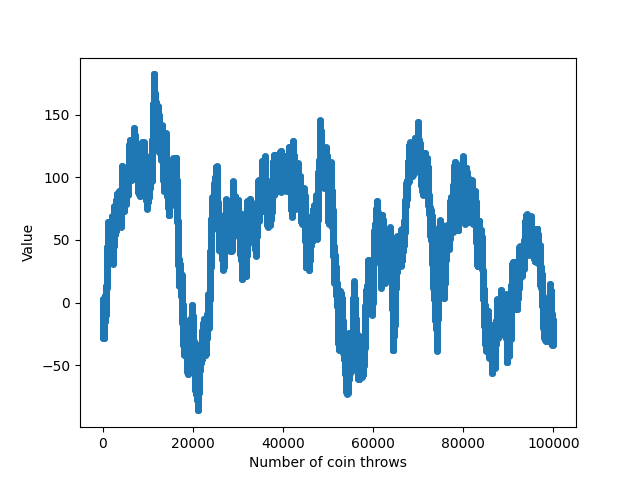
\includegraphics[scale=0.7]{./matplotlib_graphs/Figure_5.png}
\centering
\caption{Plot shows development of \texttt{value} for sample size of N = \autoref{fig10}0,000} \label{fig3}
\end{figure}

\begin{figure}
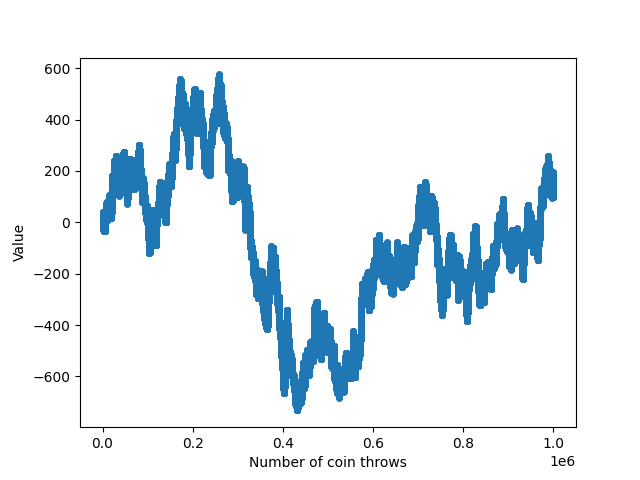
\includegraphics[scale=0.7]{./matplotlib_graphs/Figure_6.png}
\centering
\caption{Plot shows development of \texttt{value} for sample size of N = 1,000,000} \label{fig4}
\end{figure}

\begin{figure}
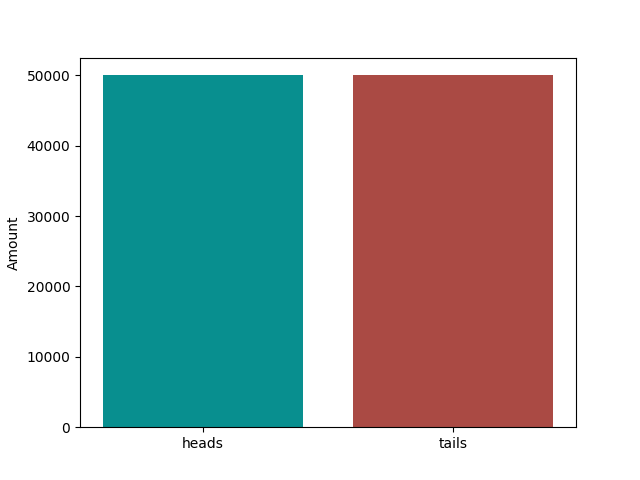
\includegraphics[scale=0.7]{./matplotlib_graphs/Figure_5_bar.png}
\centering
\caption{Bar graph shows ration of heads and tails for sample size of N = \autoref{fig10}0,000} \label{fig5}
\end{figure}

\begin{figure}
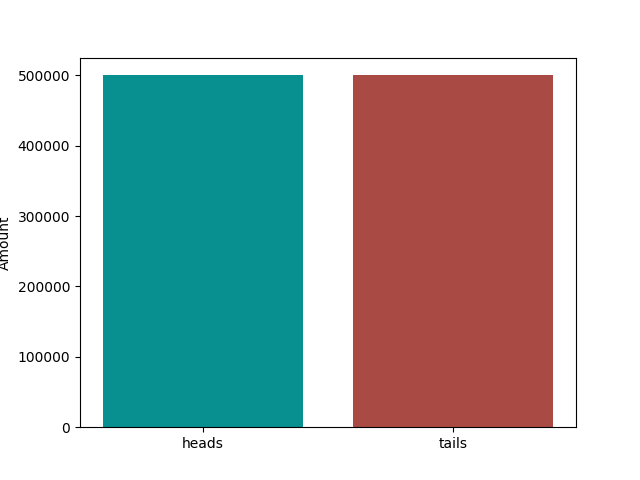
\includegraphics[scale=0.7]{./matplotlib_graphs/Figure_6_bar.png}
\centering
\caption{Bar graph shows ration of heads and tails for sample size of N = 1,000,000} \label{fig6}
\end{figure}

\begin{figure}
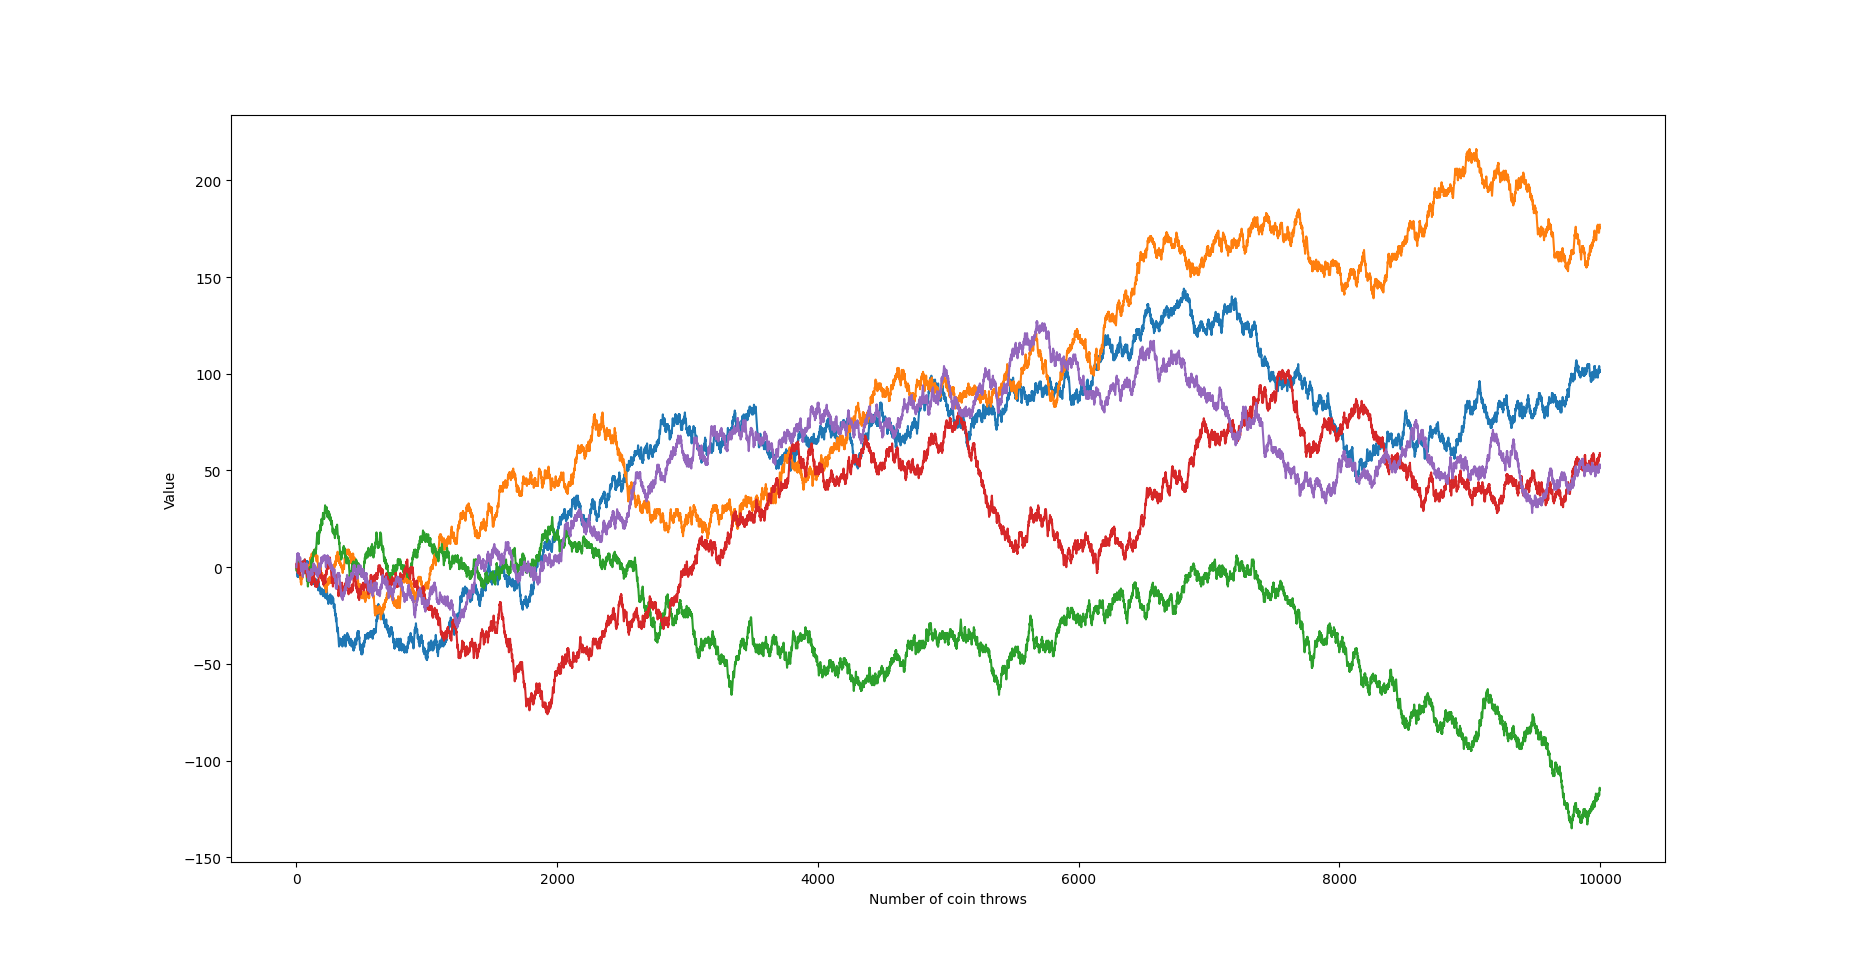
\includegraphics[scale=0.3]{./matplotlib_graphs/Figure_mult.png}
\centering
\caption{5 plots showing the development of \texttt{value} for sample size of N = \autoref{fig10}0,000} \label{fig7}
\end{figure}

\begin{figure}
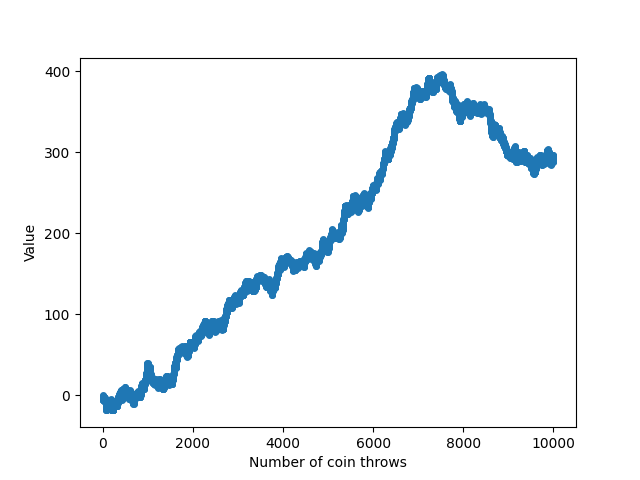
\includegraphics[scale=0.7]{./matplotlib_graphs/Figure_weighted_1.png}
\centering
\caption{Plot showing value; Probabilities: heads(0.51), tails(0.49), sample size of N = \autoref{fig10},000} \label{fig8}
\end{figure}

\begin{figure}
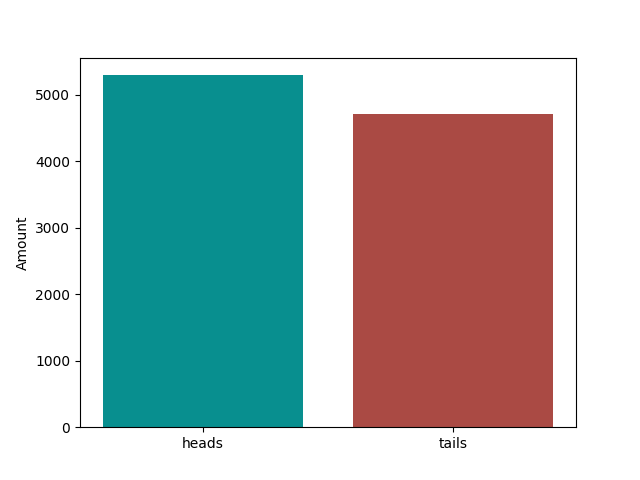
\includegraphics[scale=0.7]{./matplotlib_graphs/Figure_weighted_1_bar.png}
\centering
\caption{Bar graph showing ration; Probabilities: heads(0.51), tails(0.49), sample size of N = \autoref{fig10},000} \label{fig9}
\end{figure}

\begin{figure}
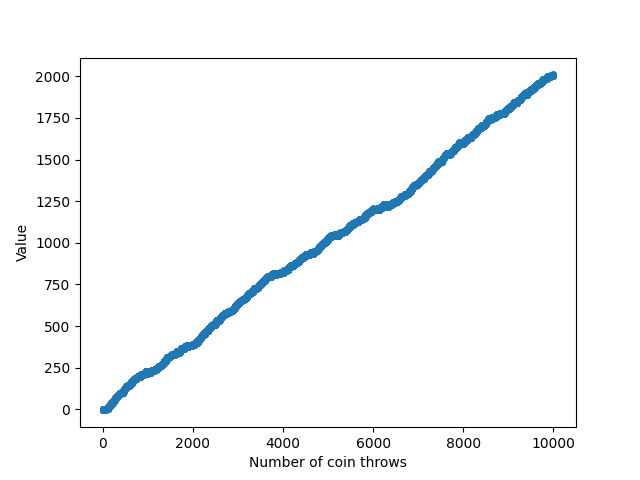
\includegraphics[scale=0.7]{./matplotlib_graphs/Figure_weighted_2.png}
\centering
\caption{Plot showing value; Probabilities: heads(0.6), tails(0.4), sample size of N = \autoref{fig10},000} \label{fig\autoref{fig10}}
\end{figure}

\begin{figure}
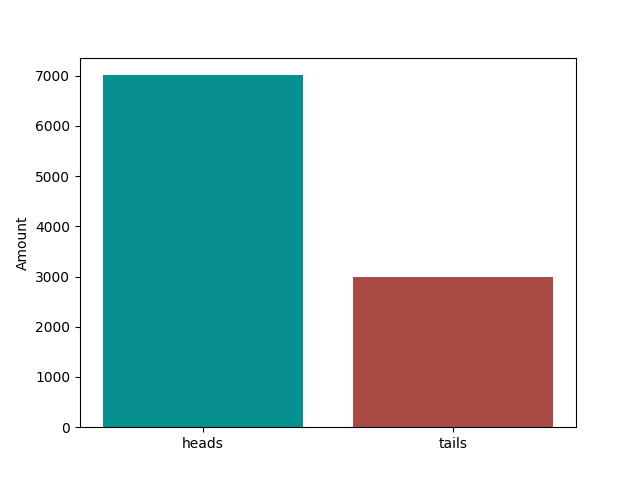
\includegraphics[scale=0.7]{./matplotlib_graphs/Figure_weighted_2_bar.png}
\centering
\caption{Bar graph showing ration; Probabilities: heads(0.6), tails(0.4), sample size of N = \autoref{fig10},000} \label{fig\autoref{fig11}}
\end{figure}

